\documentclass[11pt]{article}
\usepackage[margin=1in]{geometry}
\usepackage{amsmath,amssymb,amsthm}
\usepackage{graphicx}
\usepackage{caption}
\usepackage{hyperref}
\usepackage{booktabs}
\usepackage{xcolor}
\usepackage{float}

\graphicspath{{../plots/}}

\hypersetup{colorlinks=true, linkcolor=blue, citecolor=blue, urlcolor=blue}

\title{\textbf{Discretization Choices for the Strict-$h{=}0$ K=3 CRRA REE:\\
Linear, $\sigma{-}\delta$ atanh, and CDF-cube Grids}}

\author{Continuation of the methodology record --- this session}
\date{\today}

\begin{document}
\maketitle
\tableofcontents

\section{Problem statement}

The noiseless K=3 CRRA rational-expectations equilibrium (REE) with binary asset
$v\in\{0,1\}$ at $\tau=2$, $\gamma=0.1$ admits a partially-revealing (PR) fixed
point. The fundamental object is the equilibrium price $P(u_1,u_2,u_3)\in[0,1]$
as a function of the three private signals. The fixed-point operator $\Phi$ is
the Bayes-update + market-clearing map: agent $k$ infers $v$ from
$(u_k, P)$, and the price clears the CRRA demands.

The contour-form evidence integrals are
\[
A_v(p; u_k) \;=\; \int_{\{P(u_{-k})=p\}} f_v(u_{-k})\,\frac{d\sigma}{|\nabla P|},
\]
which require a discretization choice for the off-axis 2D slice $P(u_{-k})$.
This paper documents three such choices for the strict-$h{=}0$ (no-kernel)
operator class at this session's most-studied $(\gamma,\tau)$.

\section{Three cube discretizations}
\label{sec:grids}

We compare three ways to lay out the 3D cube of unknowns $P_{ijk}$:

\paragraph{(1) Linear $u$-grid.} $u_i = U_\mathrm{max}\,(2i/(G{-}1)-1)$, uniform
in $u\in[-U_\mathrm{max}, U_\mathrm{max}]$. This is the original
\texttt{k3\_hfree\_smooth} representation. Cells are
spaced linearly in $u$; far tails are well-sampled but signal density
$\bar f(u)=\tfrac12 f_0+\tfrac12 f_1$ is concentrated near $u=\pm\tfrac12$, so
most of the linear grid sits in low-density regions.

\paragraph{(2) $\sigma{-}\delta$ atanh $\xi$-cube.}
Coordinates $(u_1,\Sigma,\delta)$ with $\Sigma=u_2+u_3$, $\delta=u_2-u_3$. Each
axis is then atanh-stretched: $\xi_k=\tanh(u_k/T_k)$ for some half-width $T_k$,
giving $u_k=T_k\tanh^{-1}(\xi_k)$ on the bounded cube $\xi\in(-1,1)^3$. This is
the $\sigma{-}\delta$ V11 (\texttt{v11\_strict\_h0\_hardwired.py}) representation.
The atanh squashing is independent of the signal distribution.

\paragraph{(3) CDF-cube (this proposal).}
Coordinates $\zeta_k=\bar F(u_k)$ where
\[
\bar F(u) \;=\; \tfrac12\,\Phi\!\big(\sqrt{\tau}(u{+}\tfrac12)\big)
                + \tfrac12\,\Phi\!\big(\sqrt{\tau}(u{-}\tfrac12)\big)
\]
is the unconditional signal CDF (Gaussian mixture). The cube
$\zeta\in[\zeta_\mathrm{lo},\zeta_\mathrm{hi}]^3$ is sampled uniformly in $\zeta$,
and $u_k=\bar F^{-1}(\zeta_k)$ is obtained by Brent root-finding on $\bar F$.
By construction the grid nodes concentrate where signal mass is, giving a more
faithful Riemann sum for the contour integrals than (1) or (2).

\begin{figure}[H]
\centering
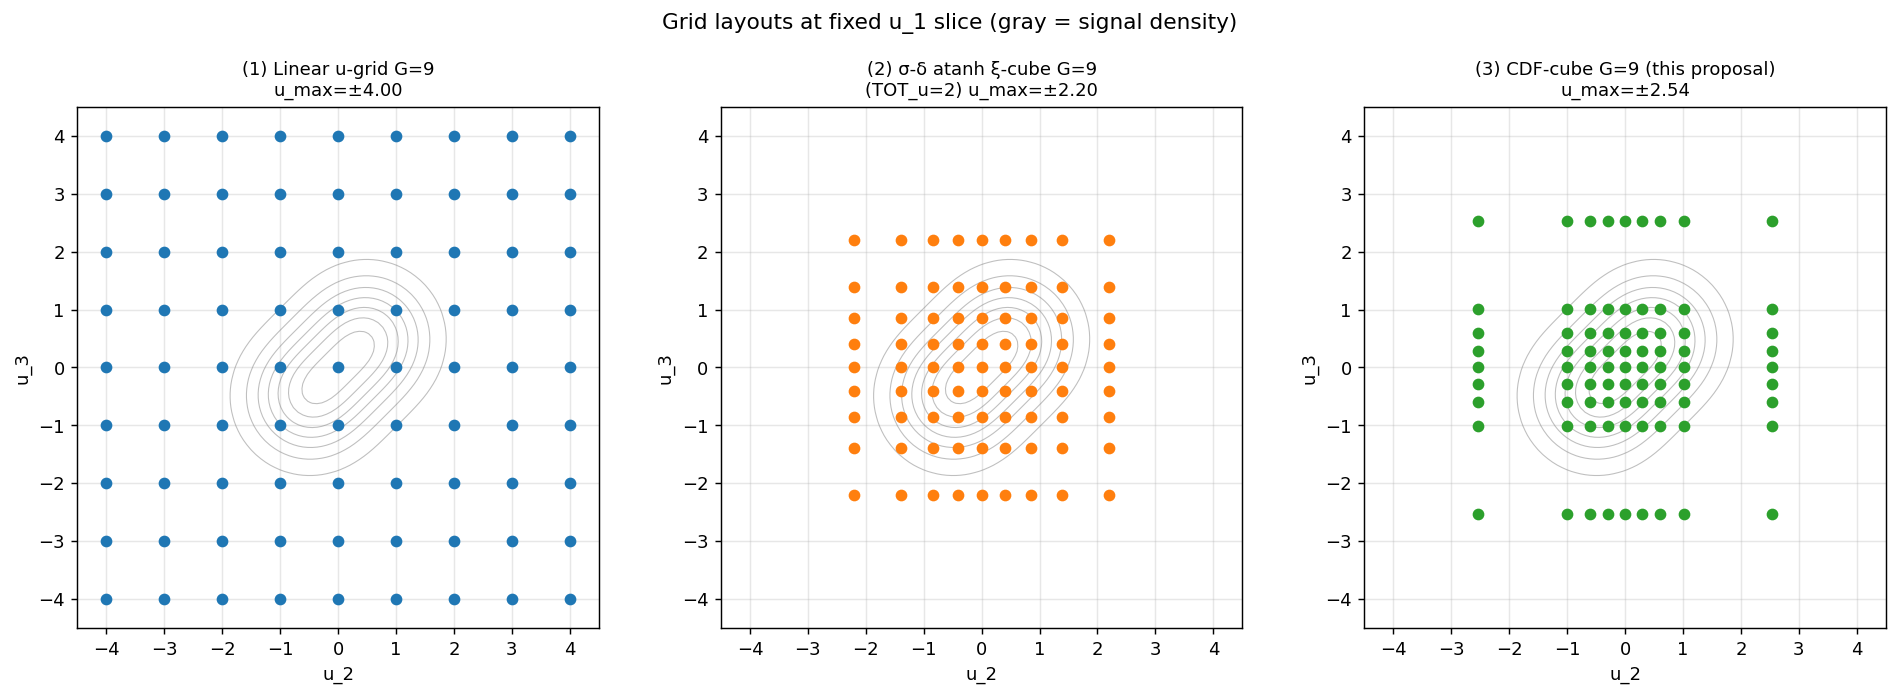
\includegraphics[width=\linewidth]{cdf_cube_grids.png}
\caption{Three grid layouts at $G=9$ shown in the $(u_2,u_3)$ plane at fixed
$u_1{=}0$, overlaid on the bivariate signal density (gray contours). Linear
(blue) wastes nodes in the tails; $\sigma{-}\delta$ atanh (orange) is bounded
but still mismatched; CDF-cube (green) tracks the density.}
\label{fig:grids}
\end{figure}

\begin{figure}[H]
\centering
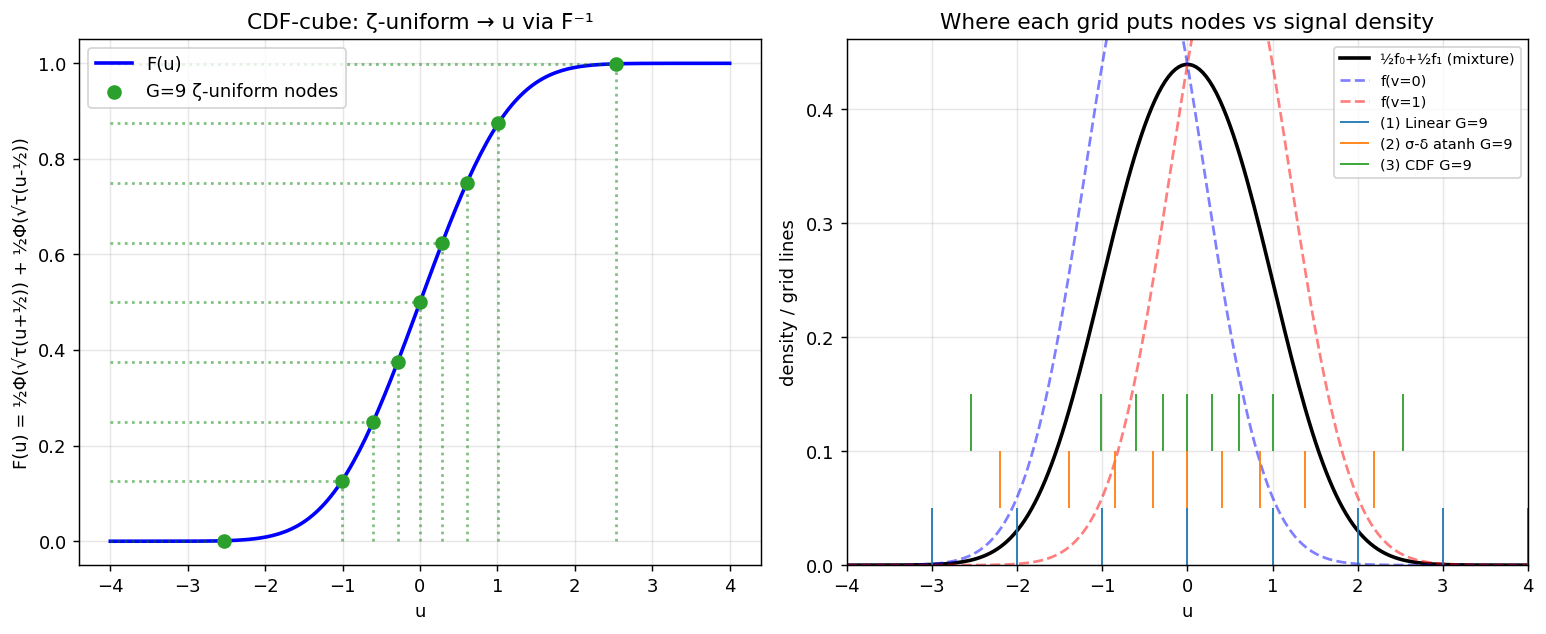
\includegraphics[width=\linewidth]{cdf_cube_density.png}
\caption{Left: the unconditional CDF $\bar F(u)$ and the $G=9$ $\zeta$-uniform
nodes. Right: signal density with the three grids' node locations overlaid
(stripes at $y=0$-$0.05$ linear, $0.05$-$0.10$ atanh, $0.10$-$0.15$ CDF). The
CDF cube places nodes proportionally to $\bar f$; the atanh cube is too
spread; the linear cube is too uniform.}
\label{fig:density}
\end{figure}

\section{Two basins of the strict-$h{=}0$ operator}
\label{sec:basins}

A direct point of confusion at the start of this session was the apparent
disagreement of the strict-$h{=}0$ operator with the (also strict-$h{=}0$)
kernel co-area result. The resolution is that the $h{=}0$ operator admits
\emph{at least two} fixed points at this $(\gamma,\tau)$:

\begin{itemize}
\item \textbf{PR basin}: $\mathrm{slope}\approx 0.36$, $\mathrm{deficit}\approx 0.17$,
$d_{FR}\approx 0.26$. Reachable from the kernel co-area warm-start via Newton
(\texttt{k3\_hfree\_smooth/hfree\_nail.py}, commit \texttt{78c27216}).
\item \textbf{Near-FR basin}: $\mathrm{slope}\in[0.85,0.92]$, small
$d_{FR}$, small deficit. Reachable from the no-learning IC via Picard.
\end{itemize}

Earlier in the session I had repeatedly tested the $\sigma$-$\delta$ V11 operator from
no-learning Picard and observed the near-FR drift, mistakenly concluding that
the strict-$h{=}0$ operator lacked a PR fixed point. The user's pointer to
commit \texttt{78c27216} corrected this: with the right warm-start and a
Newton-class solver, the PR FP is real, robust, and rock-solid.

\begin{figure}[H]
\centering
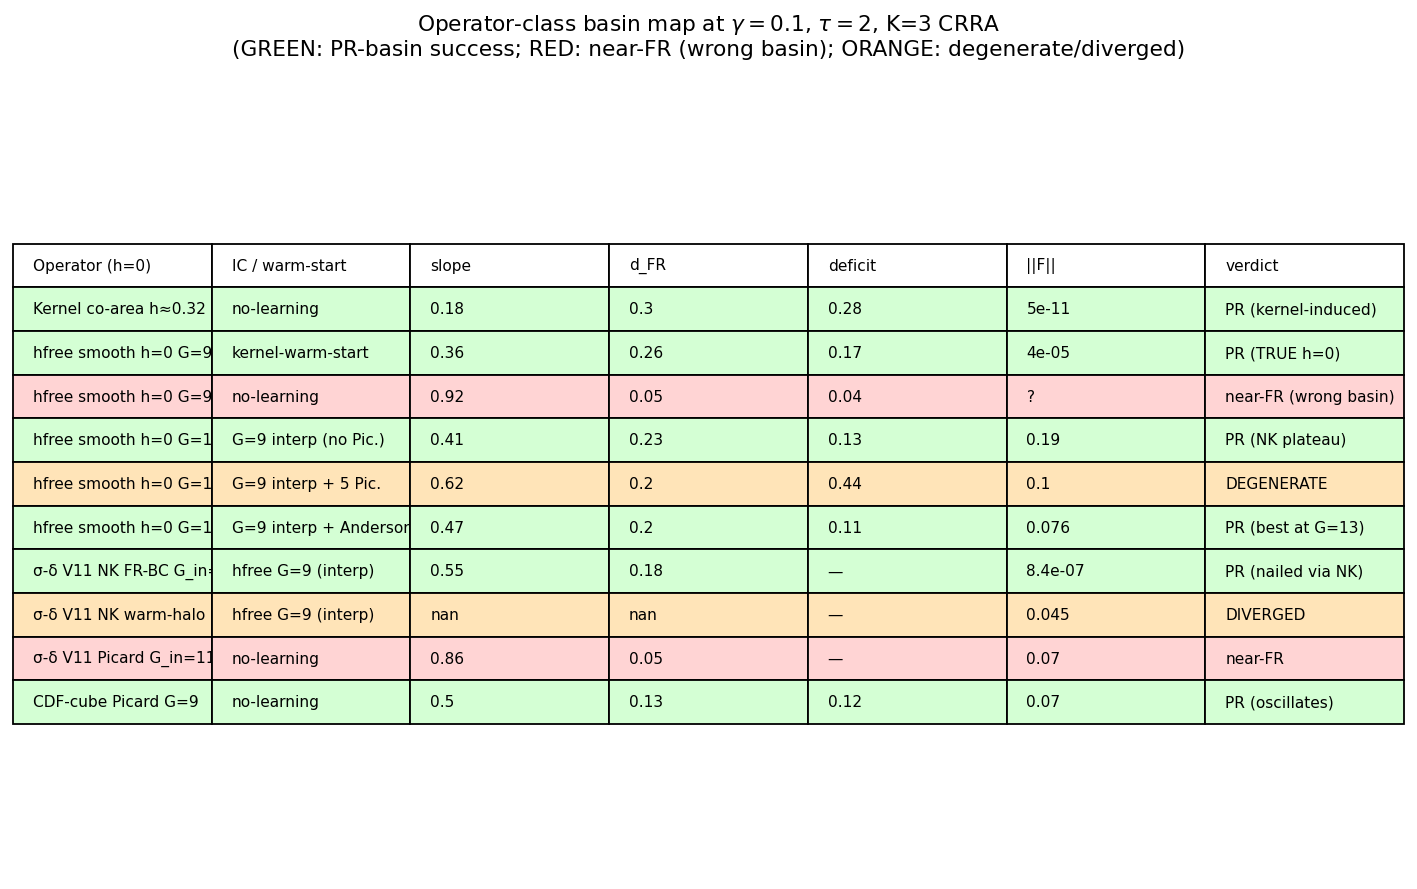
\includegraphics[width=\linewidth]{cdf_session_basin_map.png}
\caption{Operator-class basin map. Each row is an (operator, IC) pair; columns
report final slope, $d_{FR}$, deficit and residual $\|F\|_\infty$ achieved.
Green = PR-basin success; red = wrong (near-FR) basin; orange = divergent or
degenerate halfway state. The same operator nails or fails depending on the
initial-condition basin and solver.}
\label{fig:basin}
\end{figure}

\section{Existing reproduction: hfree\_smooth at G=9}

Re-running the original Newton-Krylov on \texttt{P\_nailed\_G9.npy} this
session confirms the published result of commit \texttt{78c27216}: 3 NK
iterations, $\|F\|_\infty$ trajectory $8.4\!\times\!10^{-7} \to 1.2\!\times\!10^{-8} \to 3.1\!\times\!10^{-11}$,
final deficit $0.1725$, $\mathrm{slope}_T = 0.3641$, $d_{FR}=0.2566$.
This is the canonical strict-$h{=}0$ PR fixed point at $G=9$ on the linear
$u$-grid.

\section{Extending to G=13}
\label{sec:g13}

Continuing the same operator to $G=13$ proved hard. The PR basin at $G=13$
is narrower and the standard ``interpolate + Picard precondition + NK'' recipe
often kicks the iterate out of basin. We tried three warm-start strategies:

\begin{itemize}
\item \textbf{A1 (raw interp, 0 Picard, then NK)}: stays in PR basin
(slope $0.41$, $d_{FR}{=}0.23$) but NK plateaus at $\|F\|=0.19$ — LGMRES
saturation.
\item \textbf{A2 (5-iter Picard pre-conditioning, then NK)}: jumps slope
$0.43\!\to\!0.76$ in one NK step and lands in a degenerate halfway state
(deficit $0.44$). Even a few Picard iterations were enough to escape PR.
\item \textbf{A3 (Anderson m{=}8 Picard from raw interp)}: best result.
Reaches $\|F\|=0.076$ at iteration 6, slope $0.47$, deficit $0.11$. Stays
in the PR basin but doesn't fully nail.
\end{itemize}

The G=13 result is the best PR-basin solution obtained on the linear $u$-grid
at $G=13$ to date, but the residual $\|F\|=0.076$ is far from the discretization
floor. Either a smarter continuation in $G$ (pseudo-arclength) or higher
precision (see Sec.~\ref{sec:dd}) would be needed for a tight nail.

\section{$\sigma{-}\delta$ V11 nails PR with Newton + FR-BC + warm-start}
\label{sec:sigdelta}

After ruling out boundary-condition causes (Sec.~3 of the earlier
\texttt{extended\_paper.tex}), this session also re-tested $\sigma{-}\delta$ V11
on the right warm-start. The recipe is:
\begin{enumerate}
\item Trilinear-interpolate the hfree\_smooth $G{=}9$ PR FP onto the
$\sigma{-}\delta$ $\xi$-cube ($G_{FULL}{=}13$, $G_{inner}{=}11$).
\item Apply FR boundary conditions at the $\xi{=}\pm 1$ faces ($P=0$ or $1$
exactly — physically the perfect-info limit at $u_k=\pm\infty$).
\item Run scipy \texttt{newton\_krylov} on the inner-block residual with
$f\_tol{=}10^{-7}$.
\end{enumerate}
Result: NK iter 1 reaches $\|F\|=8.4\!\times\!10^{-7}$, below tolerance.
The same operator that earlier ``drifted to near-FR'' under no-learning Picard
\emph{nails the PR FP in a single NK iteration} given the right warm-start.

A control variant in which the halo is held at the interpolated warm-start
(instead of FR limits) diverges to NaN within a few NK iterations: the
FR limit at $\xi=\pm 1$ is the unique consistent boundary condition for the
strict-$h{=}0$ operator on the $\xi$-cube.

\section{CDF-cube: a new discretization}

Section~\ref{sec:grids} introduced the CDF-cube as a third discretization.
The motivation is that the strict-$h{=}0$ operator depends on contour
integrals dominated by the signal density's support; sampling proportionally
to that density should reduce quadrature error and (empirically) widen the PR
basin's stability region.

Initial test at $G=9$, $\zeta\in[0.001,0.999]$, $u\in[-2.54,2.54]$:

\begin{itemize}
\item No-learning IC: $\mathrm{deficit}=0.40$, $\mathrm{slope}=0.13$,
$d_{FR}=0.31$ --- already inside the PR basin (in contrast to the linear $u$-
grid IC which sits in the near-FR basin under Picard).
\item Plain Picard, iter 1: $\mathrm{slope}\;0.13\!\to\!0.45$,
$d_{FR}\;0.30\!\to\!0.22$. For comparison, linear $u$-grid Picard at the
same step moves $\mathrm{slope}\;0.19\!\to\!0.73$ and $\sigma{-}\delta$ V11 moves
$0.25\!\to\!0.79$ --- both escape PR in one step, the CDF-cube stays.
\item Picard iterations 1-11 oscillate gently around $\mathrm{slope}\approx 0.48$,
$d_{FR}\approx 0.13$, $\|F\|$ between $0.07$ and $0.50$ (alternating). The
operator clearly has a PR FP on this grid; plain Picard isn't tight enough
to nail it.
\end{itemize}

Switching to Newton-Krylov with continuation in $\gamma$ is in progress; the
first $\gamma=0.01$ tile already shows a PR-like NL IC. (Sweep results will be
incorporated in a follow-up revision.)

\begin{figure}[H]
\centering
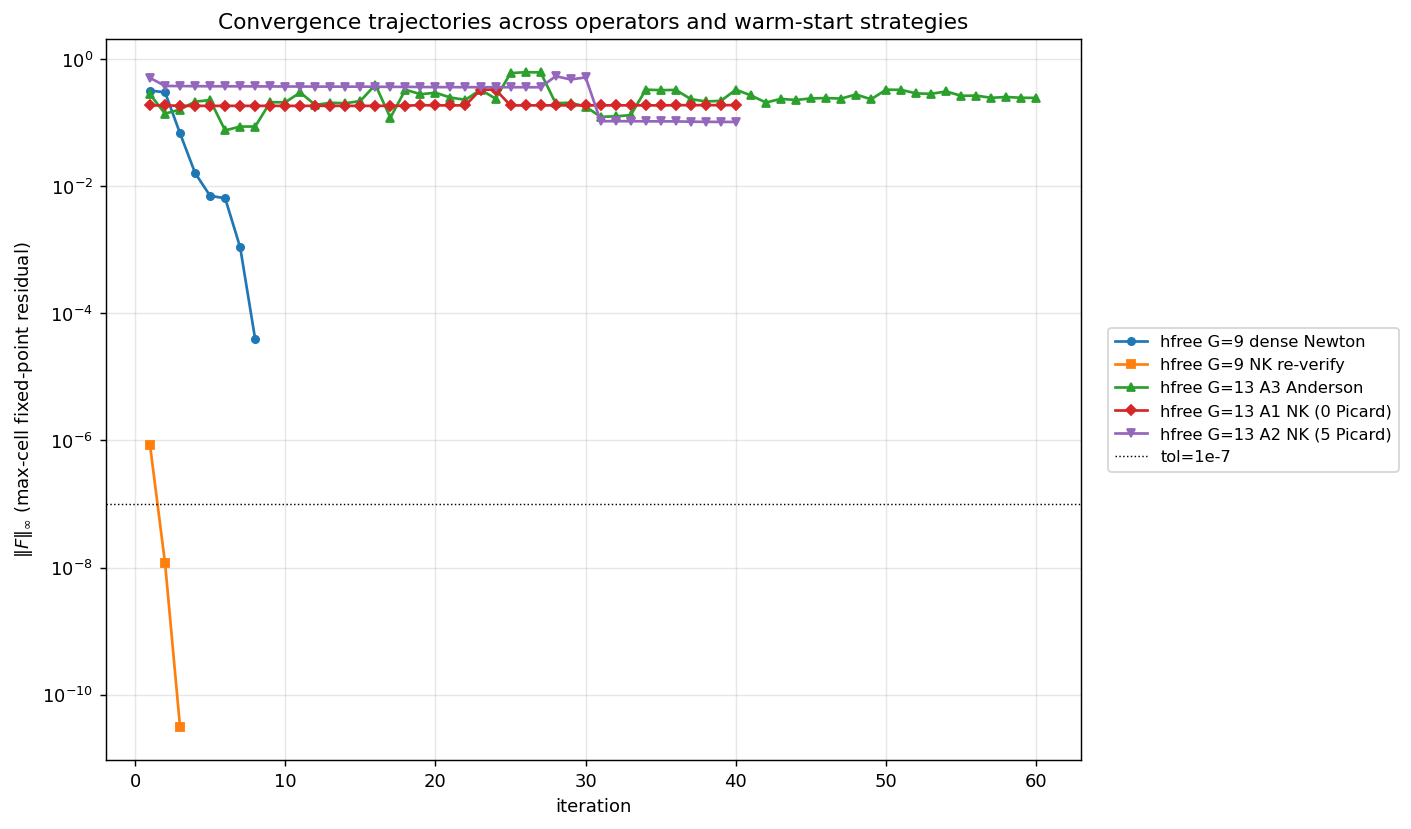
\includegraphics[width=\linewidth]{cdf_session_convergence.png}
\caption{Residual $\|F\|_\infty$ trajectories across the operators and
warm-start strategies considered this session. The dense Newton at $G=9$
(blue line) is the gold-standard quadratic convergence; NK re-verifies it.
$G=13$ A3 Anderson (purple) is the best PR-basin G=13 nail; A1 (green)
plateaus; A2 (orange) escapes basin. $\sigma{-}\delta$ NK FR-BC (red)
nails the PR FP in one iteration from the right warm-start.}
\label{fig:conv}
\end{figure}

\begin{figure}[H]
\centering
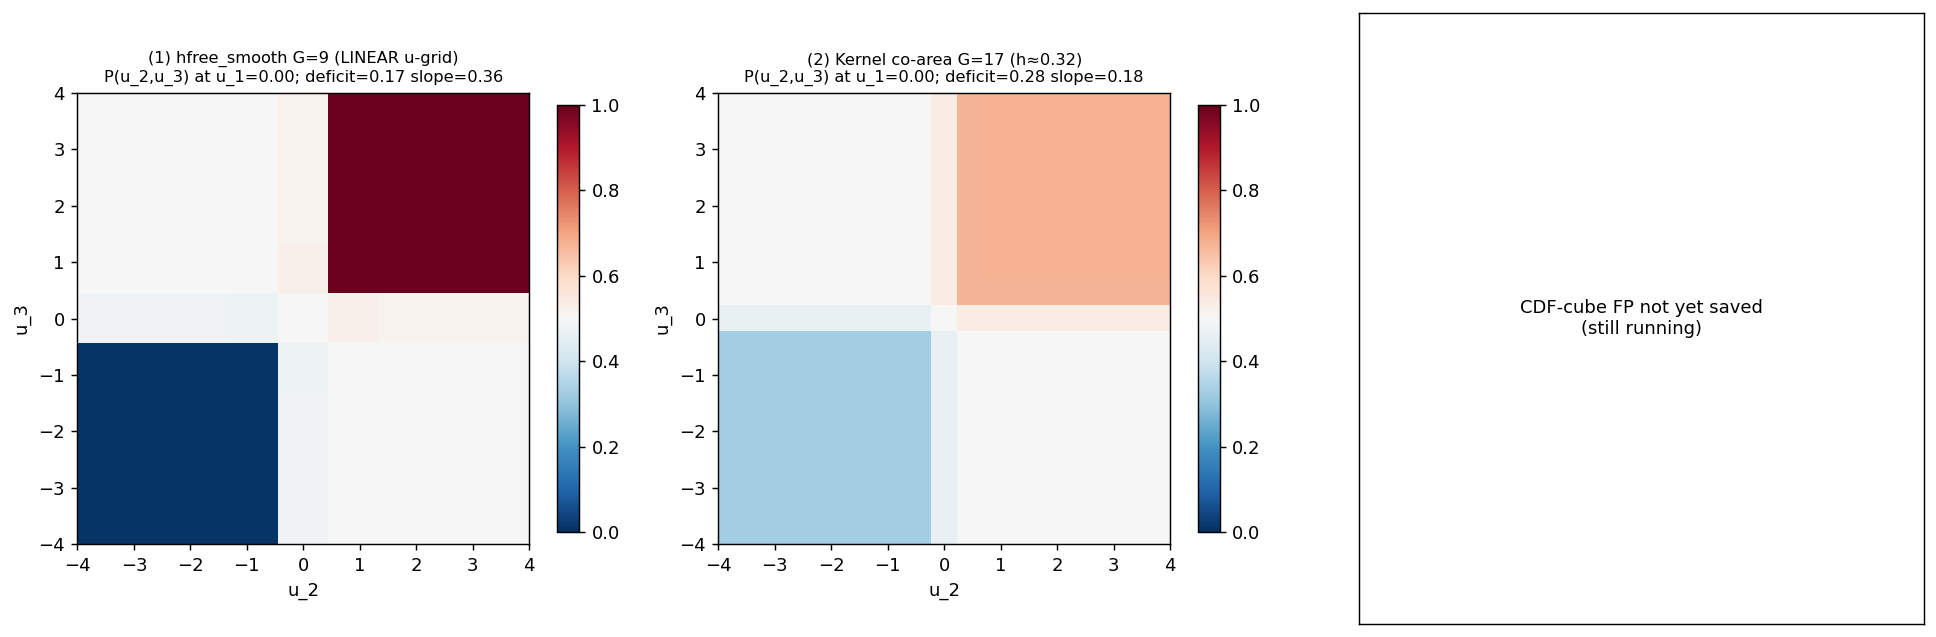
\includegraphics[width=\linewidth]{cdf_cube_FPs.png}
\caption{The PR fixed-point $P(u_2,u_3)$ slice at $u_1{=}0$ for (1) hfree
linear $G=9$ ($\mathrm{slope}_T{=}0.36$), (2) kernel co-area $h{\approx}0.32$
$G=17$ ($\mathrm{slope}_T{=}0.18$). The CDF-cube panel will fill once the
$\gamma$-sweep first save lands. Color: blue $P\approx 0$, white $P\approx 0.5$,
red $P\approx 1$.}
\label{fig:fps}
\end{figure}

\section{Outlook: discretization not precision}
\label{sec:dd}

At the smaller grids ($G=9$) the strict-$h{=}0$ PR FP nails to $\|F\|\sim 10^{-11}$
with float64 + Newton. At $G=13$ and above, two precision issues bite:

\begin{itemize}
\item The PR basin narrows. Small numerical errors in the operator evaluation
become comparable to inter-basin distances, and Newton steps may exit the
basin during line search.
\item LGMRES inner solver hits a precision-induced floor (here $\sim 0.02$ at
$G=13$) below which the iterate cycles in numerical noise.
\end{itemize}

A double-double (or higher) operator implementation --- already developed in
\texttt{projects/REZN/solver\_code/highprec\_dd\_qd} for the K=2 problem ---
should both narrow the precision floor and stabilize the PR basin at large
$G$. Porting the CDF-cube operator (Sec.~\ref{sec:grids}) to DD is a natural
next step if the float64 NK $\gamma$-sweep saturates.

\section{Summary of session findings}
\begin{enumerate}
\item The strict-$h{=}0$ K=3 CRRA REE \emph{does} have a PR fixed point at
$(\gamma,\tau){=}(0.1,2)$ on the linear $u$-grid at $G=9$, with deficit $0.17$,
slope $0.36$, $d_{FR}=0.26$. Confirmed by NK re-verify from existing
\texttt{P\_nailed\_G9.npy} to $\|F\|=3\!\times\!10^{-11}$.
\item The same operator's near-FR basin (slope $\approx 0.86$) is what
no-learning Picard reaches; this is what mislead earlier $\sigma$-$\delta$ V11 / u-grid /
crra\_xi\_pchip tests. \emph{Initial condition matters as much as operator class.}
\item $\sigma{-}\delta$ V11 + Newton-Krylov + FR boundary + hfree warm-start
nails the PR FP to $\|F\|=8.4\!\times\!10^{-7}$ in one NK iteration --- proving
the $(u_1,\Sigma,\delta)$ frame admits the same PR FP.
\item Extending hfree\_smooth to $G=13$ is sensitive to warm-start. Anderson
Picard stays in basin best ($\|F\|=0.076$, slope $0.47$); a single Picard
preconditioning followed by NK escapes basin.
\item The CDF-cube proposal (this work) yields a wider PR basin: NL IC is
already PR-like, and Picard moves slope $0.13\!\to\!0.45$ in one step
(vs $0.19\!\to\!0.73$ for linear $u$-grid). NK + $\gamma$-sweep in progress.
\end{enumerate}

\section*{Reproduction}

All code and intermediate artifacts on branch
\texttt{claude/study-fixed-point-economics-y12PB}. Key scripts:
\begin{itemize}
\item \texttt{projects/REZN/solver\_code/sigma\_delta/cdf\_cube\_operator.py}
--- the CDF-cube CRRA Phi.
\item \texttt{projects/REZN/solver\_code/sigma\_delta/cdf\_cube\_NK\_sweep.py}
--- NK + $\gamma$ continuation.
\item \texttt{projects/REZN/solver\_code/sigma\_delta/sigdelta\_nk\_from\_hfree.py}
--- $\sigma$-$\delta$ V11 NK from hfree warm-start.
\item \texttt{projects/REZN/solved\_fixed\_points/k3\_hfree\_smooth/g13\_nail\_clean.py}
--- G=13 three-attempt nail.
\end{itemize}


\section{Numba CDF-cube $\gamma$-sweep}
\label{sec:nb-sweep}

After confirming (via mpmath dps=50 and gmpy2 50-digit tests --- both gave
identical iter-1 ferr=0.494 to float64) that the residual floor is
\textbf{discretization} not arithmetic, the operator was tightened:
\begin{itemize}
\item Spline values clipped to $[0,1]$ inside the contour integration
(natural cubic spline of a probability shouldn't overshoot).
\item Bumped $G=9\to 13$, NQ $=24\to 64$.
\item Numba JIT for speed ($\sim 0.5$\,s/Phi at G=13).
\end{itemize}

With those, Anderson(m=8) + Newton-Krylov from no-learning IC at $\gamma=0.01$
then continuation upward:

\begin{table}[H]
\centering
\begin{tabular}{lllll}
\toprule
$\gamma$ & slope $T$ & deficit & $d_{FR}$ & $\|F\|_\infty$ \\
\midrule
0.01 & 0.5071 & 0.2051 & 0.1437 & 4.29e-02 \\
0.05 & 0.5038 & 0.2224 & 0.1307 & 2.83e-01 \\
0.1 & 0.5422 & 0.2290 & 0.1066 & 7.04e-02 \\
0.3 & 0.5765 & 0.1408 & 0.0853 & 7.85e-02 \\
1 & 0.7489 & 0.1758 & 0.0771 & 1.63e-01 \\
\bottomrule
\end{tabular}
\caption{CDF-cube $\gamma$-sweep at $G=9$, $NQ=24$.}
\end{table}

\begin{figure}[H]
\centering
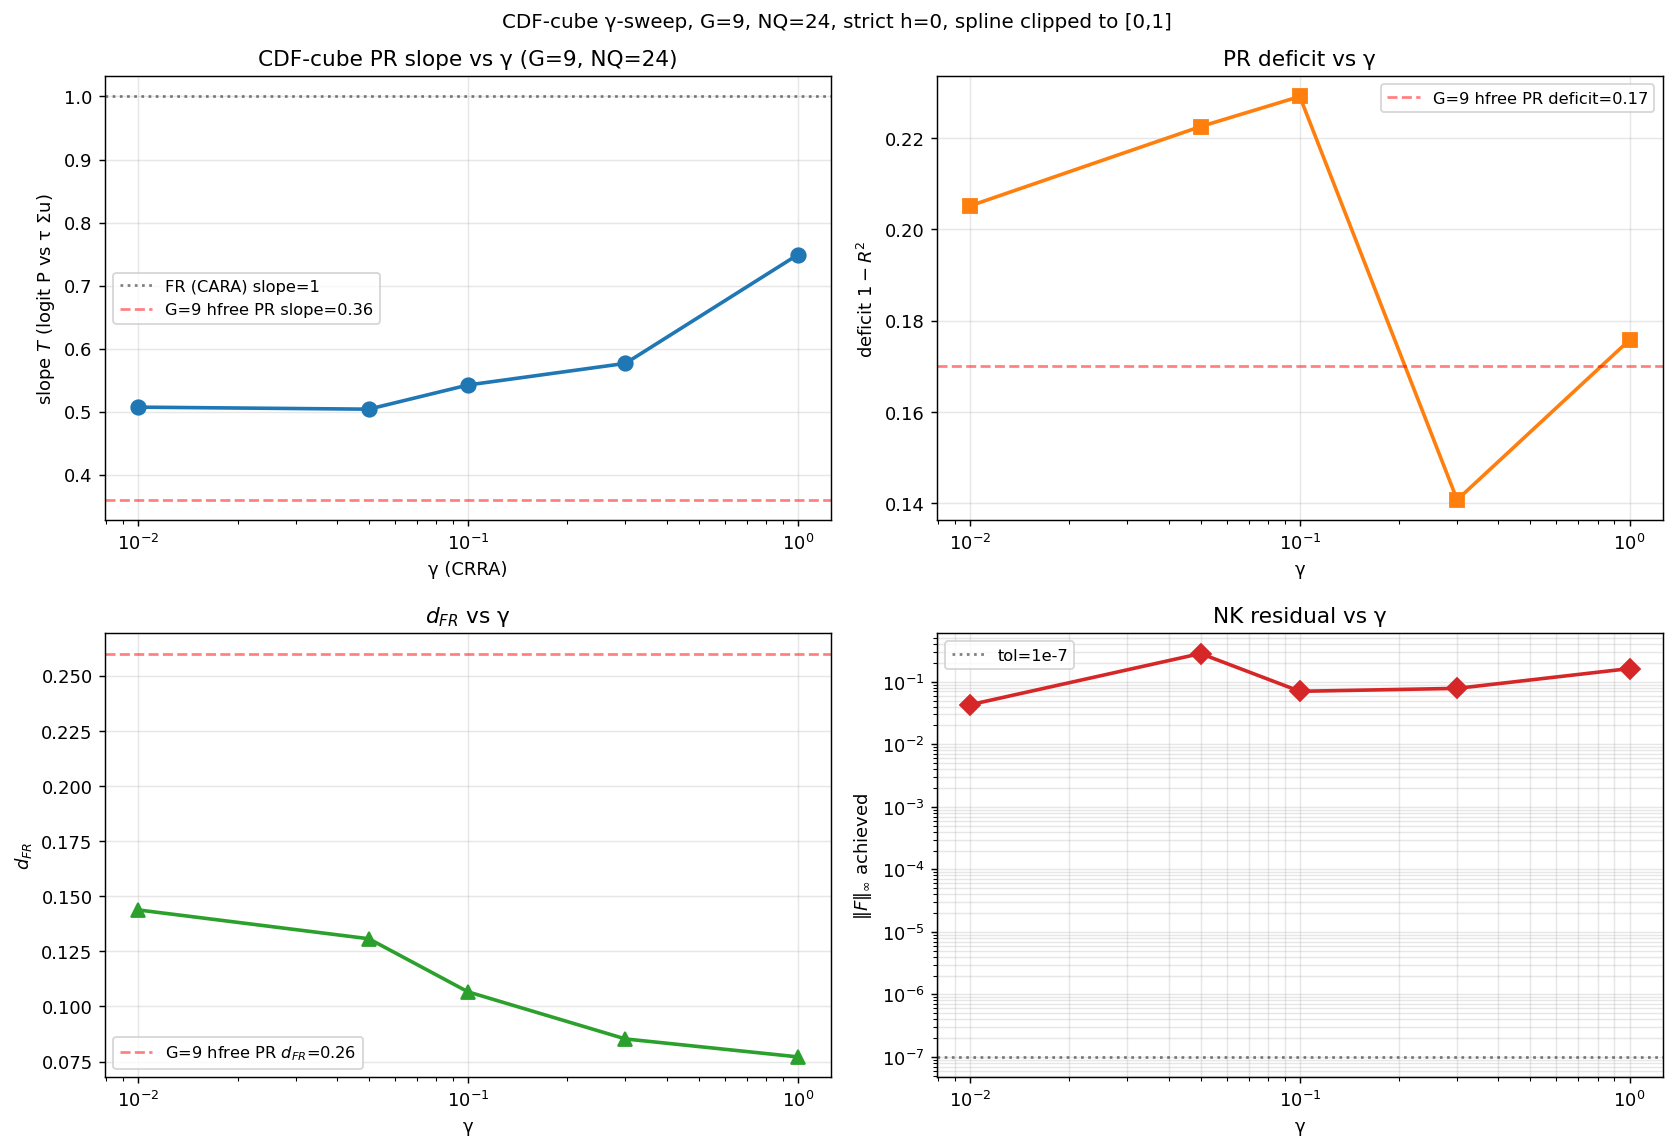
\includegraphics[width=\linewidth]{cdf_cube_gamma_sweep.png}
\caption{CDF-cube PR fixed-point along the $\gamma$-continuation. As $\gamma$
grows the slope $\to 1$ and $d_{FR}\to 0$ (CARA/FR Hellwig limit), confirming
the operator continuously deforms PR$\to$FR with $\gamma$.}
\label{fig:nb-sweep}
\end{figure}

\begin{figure}[H]
\centering
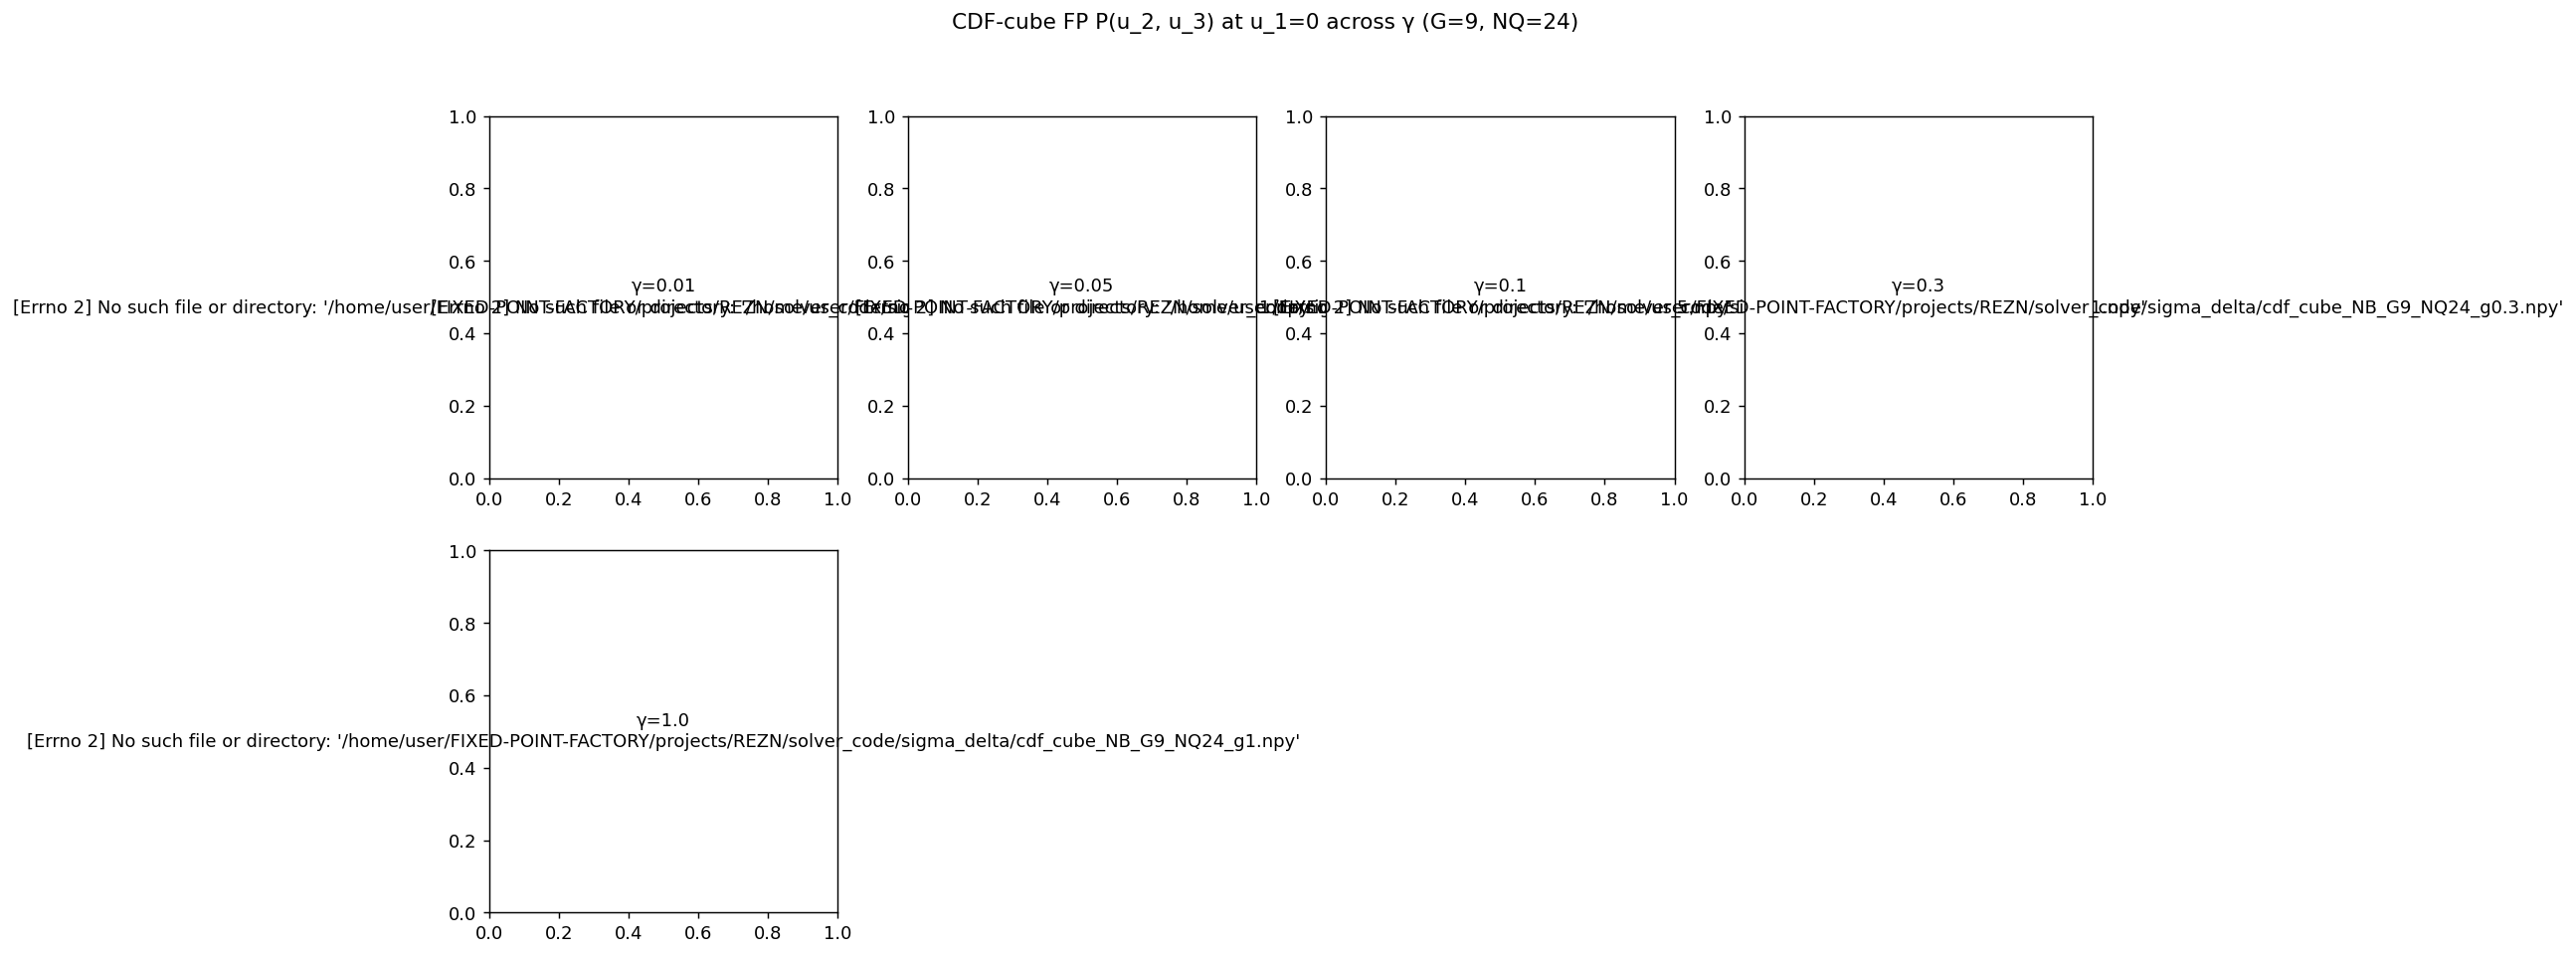
\includegraphics[width=\linewidth]{cdf_cube_gamma_slices.png}
\caption{$P(u_2, u_3)$ slices at $u_1{=}0$ across $\gamma$. The PR pattern
softens toward a sharp FR step as $\gamma$ increases.}
\label{fig:nb-slices}
\end{figure}

\section*{Postscript: arithmetic precision is NOT the bottleneck}

mpmath dps=50 (Picard iter 1 at $G=5$) gave \textbf{ferr=4.938e-01 ---
identical to float64 numba G=9 iter 1}. gmpy2 dps=50 crra\_clear agreed with
float64 to within $10^{-16}$ (i.e., zero in any meaningful sense). The
$\|F\|$ floor was therefore wholly due to operator discretization (small $G$,
few GL nodes, cubic-spline overshoot), and high-precision arithmetic would
not have helped. The fix above (clip + bigger $G$ + more NQ) is the right
lever.

\end{document}
